\subsection{L'idée initiale}
Suite à une première concertation au sein du groupe, nous avons décidé de coder une fonctionnalité qui nous permettrait de localiser des photos prises sur une carte. Après consultation avec les professeurs, nous avons ajouter à cette idée une fonctionnalité de résolution de parcours. Cette dernière, nous permet de créer une sorte de GeoGuessr. 

La fonctionnalité se décompose en deux scripts distincts :
\textit{construire\_parcours.py} pour la création du parcours, et
\textit{resoudre\_parcours.py} pour la résolution.

\subsection{Capteurs sollicités}

Quatre capteurs sont mobilisés dans cette fonctionnalité :

\begin{itemize}
    \item \textbf{Module GNSS} : fournit la position absolue du joueur en
    latitude/longitude. Utilisé à la fois lors de la construction (enregistrement
    des coordonnées des checkpoints) et lors de la résolution (estimation de
    la proximité d'un checkpoint).
    \item \textbf{IMU} : complète le GPS en temps réel via le filtre de Kalman,
    assurant une estimation de position continue entre deux fixes GPS.
    \item \textbf{Caméra (RPi Camera Module 3)} : capture des photos de
    référence lors de la construction, et des photos de vérification lors de
    la résolution. Les images sont comparées par un algorithme de mise en
    correspondance de points caractéristiques.
    \item \textbf{Buzzer} : fournit un retour audio au joueur une mélodie
    courte pour un checkpoint validé, une mélodie plus longue pour la
    complétion du parcours.
\end{itemize}

Un écran LCD et un bouton poussoir complètent l'interface utilisateur.

\subsection{Architecture logicielle}

Le script de résolution repose sur une architecture multi-threadée à trois
fils d'exécution parallèles :

\begin{itemize}
    \item \textbf{Thread GPS} : appelle \texttt{gnss\_position()} en continu
    et envoie les trames de position dans une queue partagée.
    \item \textbf{Thread IMU} : appelle \texttt{get\_imu\_data()} en continu
    et envoie les données inertielles dans la même queue.
    \item \textbf{Thread fusion} : consomme la queue, alimente le filtre de
    Kalman et met à jour la position estimée \texttt{last\_kalman\_pos}.
\end{itemize}

Le thread principal effectue un polling du bouton poussoir et déclenche la
vérification de checkpoint sur appui.

\subsection{Implémentation}

\subsubsection{Construction du parcours}

Lors de la construction, l'opérateur se déplace de point en point sur le
campus. À chaque checkpoint, il peut prendre plusieurs photos de référence
via un \textbf{appui court} (moins de 1.5 secondes) sur le bouton, puis
valider le checkpoint par un \textbf{appui long} (plus de 1.5 secondes).
La possibilité de prendre plusieurs photos de référence par checkpoint
améliore la robustesse de la validation visuelle ultérieure.

Les données sont enregistrées dans un fichier \texttt{parcours.txt} au
format suivant :

\begin{verbatim}
img1.jpg,img2.jpg;49.3845;1.0686
img3.jpg;49.3850;1.0690
\end{verbatim}

Chaque ligne correspond à un checkpoint : la liste des images de référence
séparées par des virgules, suivie des coordonnées GPS latitude et longitude.

\subsubsection{Résolution du parcours}

Au lancement, le script génère automatiquement une carte Folium affichant
les checkpoints avec leurs photos de référence en popup, permettant au joueur
de visualiser les emplacements à atteindre.

La validation d'un checkpoint se déroule en deux étapes successives :

\begin{enumerate}
    \item \textbf{Validation géographique} : sur appui bouton, la distance
    entre la position Kalman estimée et le checkpoint est calculée via la
    formule géodésique. Si cette distance est inférieure à 25 mètres, la
    vérification visuelle est déclenchée.
    \item \textbf{Validation visuelle} : une photo est capturée et comparée
    aux images de référence du checkpoint par l'algorithme ORB. Si le score
    de correspondance dépasse le seuil, le checkpoint est validé.
\end{enumerate}

Ce double critère proximité GPS \textit{et} reconnaissance visuelle
réduit les faux positifs : être proche d'un checkpoint ne suffit pas,
il faut également photographier le bon élément visuel.

\begin{figure}[htbp]
    \centering
    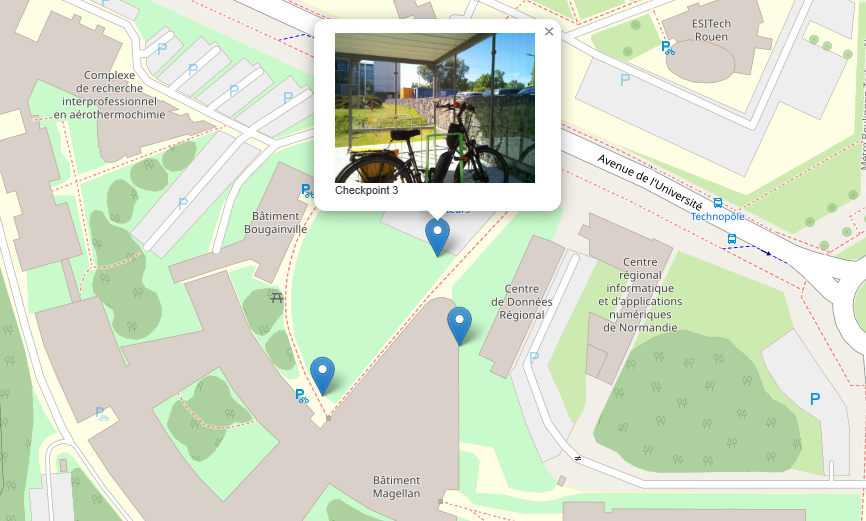
\includegraphics[width=0.85\textwidth]{images/carte_folium.png}
    \caption{Carte Folium générée au lancement de \texttt{resoudre\_parcours.py}
    les marqueurs indiquent les checkpoints du parcours. Au clic, une popup
    affiche la photo de référence à retrouver.}
    \label{fig:carte_folium}
\end{figure}

\subsubsection{Fusion GPS/IMU en temps réel}

La position du joueur est estimée en continu par un filtre de Kalman
fonctionnant selon le modèle à vitesse constante décrit en
section~\ref{sec:ekf}. Les paramètres sont identiques à ceux calibrés
pour la Partie 1 :

\begin{equation}
    R = \begin{bmatrix} 1.20 & 0 \\ 0 & 0.07 \end{bmatrix} \text{ m}^2,
    \qquad \sigma_a = 0.86 \text{ m/s}^2
\end{equation}

\subsubsection{Validation visuelle par ORB}

L'algorithme ORB (\textit{Oriented FAST and Rotated BRIEF}) est un
détecteur de points caractéristiques invariant aux rotations et aux
changements d'échelle. Pour chaque paire d'images, il extrait jusqu'à
2000 points d'intérêt et calcule leurs descripteurs binaires. La mise
en correspondance est effectuée par un \texttt{BFMatcher} à distance de
Hamming, avec filtre à distance inférieure à 50.

Lorsque plusieurs images de référence sont disponibles pour un checkpoint,
le meilleur score parmi toutes les comparaisons est retenu :

\begin{equation}
    \text{score} = \min\left(\frac{N_{\text{matches}}}{2000} \times 100,\ 100\right) \%
\end{equation}

Le checkpoint est validé si le nombre de correspondances dépasse
$N_{\text{min}} = 400$. Ce seuil a été fixé expérimentalement.


\subsubsection{Fonctionnement détaillé de l'algorithme ORB}

ORB (\textit{Oriented FAST and Rotated BRIEF}) est un algorithme de
détection et description de points caractéristiques, développé comme
alternative rapide à SIFT et SURF. Il se compose de deux étapes
successives.

\paragraph{Détection des points clés}
FAST (\textit{Features from Accelerated Segment Test}) identifie les
points d'intérêt dans une image en analysant l'intensité des pixels
sur un cercle de 16 pixels autour de chaque candidat. Un point est
retenu comme coin si un arc suffisamment long de pixels consécutifs
est significativement plus clair ou plus sombre que le pixel central.
ORB ajoute à FAST une composante d'orientation : un gradient d'intensité
local est calculé pour attribuer un angle à chaque point détecté, rendant
le descripteur invariant aux rotations.

\paragraph{Description}
BRIEF (\textit{Binary Robust Independent Elementary Features}) représente
chaque point clé par un vecteur binaire construit à partir de comparaisons
d'intensité entre paires de pixels dans un voisinage local. La version
\textit{Rotated} de ORB oriente ces comparaisons selon l'angle calculé
par FAST, garantissant ainsi l'invariance rotationnelle du descripteur.

\paragraph{Mise en correspondance}
Les descripteurs binaires sont comparés par distance de Hamming (nombre
de bits différents entre deux descripteurs). Un \texttt{BFMatcher}
(\textit{Brute-Force Matcher}) compare exhaustivement chaque descripteur
de l'image de test contre tous ceux de l'image de référence, et retient
les paires dont la distance est inférieure à 50.

\begin{figure}[htbp]
    \centering
    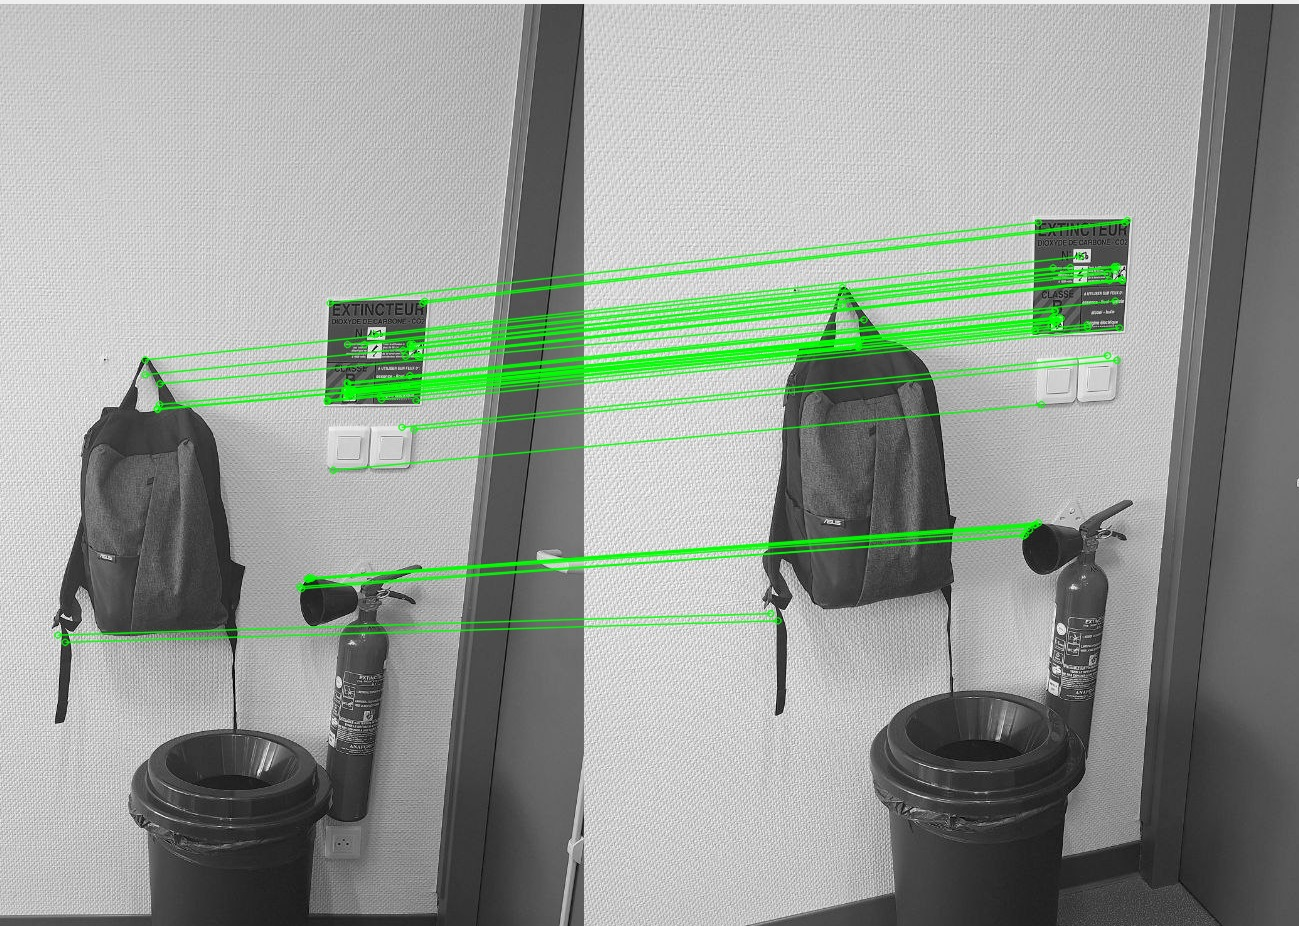
\includegraphics[width=0.95\textwidth]{images/orb_matching.jpeg}
    \caption{Visualisation des correspondances ORB entre deux photos du
    même checkpoint (image gauche : référence, image droite : vérification).
    Les lignes vertes relient les points caractéristiques mis en
    correspondance la densité et la cohérence géométrique des lignes
    indiquent une reconnaissance réussie.}
    \label{fig:orb_matching}
\end{figure}

La Figure~\ref{fig:orb_matching} illustre un cas de validation réussie :
les correspondances s'établissent sur des éléments texturés stables
(extincteur, panneau mural, interrupteurs), répartis sur l'ensemble
de l'image. Cette distribution spatiale large est caractéristique
d'une vraie reconnaissance et non d'une coïncidence locale.

\subsubsection{Retour utilisateur LCD et buzzer}

À chaque action du joueur, un retour immédiat est fourni via l'écran LCD
et le buzzer. Le tableau suivant récapitule les messages affichés selon
les situations :

\begin{table}[H]
    \centering
    \caption{Messages LCD selon l'état du système}
    \begin{tabular}{ll}
        \hline
        \textbf{Situation} & \textbf{Affichage LCD} \\
        \hline
        Démarrage           & \texttt{Appuyez bouton} \\
        Capture en cours    & \texttt{Photo en cours...} \\
        Trop loin           & \texttt{Trop loin...} \\
        Photo non reconnue  & \texttt{Mauvais endroit!} + score \% \\
        Checkpoint validé   & \texttt{CP X valide !} + score \% \\
        Parcours terminé    & \texttt{Bravo ! Fini !} \\
        \hline
    \end{tabular}
\end{table}

Le score affiché correspond au pourcentage de correspondances ORB
($N_{\text{matches}} / 2000 \times 100$), permettant au joueur de savoir
s'il était proche de valider ou complètement hors sujet.

Le buzzer fournit un retour audio complémentaire : une mélodie courte signale la validation d'un checkpoint, tandis qu'une mélodie
plus longue célèbre la complétion du parcours entier. Ces signaux permettent
au joueur de jouer sans regarder l'écran en permanence.



\subsection{Outils et bibliothèques utilisés}

La fonctionnalité mobilise plusieurs outils et bibliothèques vus en ITI3 :

\begin{itemize}
    \item \textbf{threading / queue} : architecture multi-threadée pour
    l'acquisition simultanée GPS et IMU, avec synchronisation par file
    d'attente partagée paradigme de programmation concurrente vu en
    cours système.
    \item \textbf{GPIO / PWM} : contrôle du buzzer par modulation de
    largeur d'impulsion et polling du bouton poussoir, utilisés en TP
    Capteurs.
    \item \textbf{Folium} : génération de la carte interactive OpenStreetMap
    avec les checkpoints en popup.
    \item \textbf{RPLCD} : affichage du score de correspondance et des
    messages de validation sur l'écran LCD I2C en temps réel.
    \item \textbf{subprocess / rpicam-still} : déclenchement de la caméra
    RPi Camera Module 3 depuis Python pour la capture des photos.
\end{itemize}

\subsection{Analyse critique}

La fonctionnalité a été testée sur le campus avec des parcours de 3 à 5
checkpoints. Les résultats sont globalement satisfaisants : les checkpoints
étaient retrouvés et validés correctement, avec une fiabilité variable selon
les conditions.

Plusieurs limitations ont été identifiées :

\begin{enumerate}
    \item \textbf{Dépendance à la vitesse de marche} : le modèle cinématique
    à vitesse constante du filtre de Kalman suppose un déplacement régulier.
    Une marche rapide dégrade la précision de l'estimation de position entre
    deux fixes GPS, ce qui peut empêcher la détection de proximité à 25 mètres.
    En pratique, un rythme de marche modéré était nécessaire pour un
    fonctionnement fiable.

    \item \textbf{Sensibilité aux conditions d'éclairage} : l'algorithme ORB
    est sensible aux variations d'éclairage entre la phase de construction et
    la phase de résolution. Un changement de luminosité important (ciel couvert
    vs ensoleillé) réduit le nombre de correspondances et peut provoquer des
    faux négatifs.

    \item \textbf{Seuil ORB empirique} : le seuil de 400 correspondances a
    été fixé par expérimentation. Il ne repose pas sur un modèle statistique
    formel, ce qui le rend potentiellement fragile face à des scènes peu
    texturées ou à des angles de prise de vue trop différents entre la
    référence et la vérification.

    \item \textbf{Seuil GPS de 25 mètres} : ce seuil est volontairement large
    pour compenser les imprécisions du GPS en extérieur. Sans la validation
    visuelle ORB, il serait insuffisant pour discriminer des checkpoints
    proches les uns des autres.
\end{enumerate}



L'utilisation conjointe de la proximité GPS et de la reconnaissance visuelle
constitue un choix de conception robuste : les deux modalités se compensent
mutuellement. Une piste d'amélioration serait de remplacer ORB par un
réseau de neurones convolutif pré-entraîné, plus robuste aux variations
d'éclairage et de point de vue.